% letztes Update: 20-Okt-19
\section*{Einleitung}

\emph{Sonderzeichen}  wie <<\& oder \%>> müssen mit einem Backslash maskiert werden, damit sie von LaTeX nicht als Befehle missverstanden werden.

\verb|<<\& oder \%>>| 

\emph{Website}

\url{https://golatex.de/wiki/Hauptseite} 

\href{https://golatex.de/wiki/Hauptseite}{deutschen GoLaTeX-Wiki}
\marginpar{www}
\begin{lstlisting}[language=TeX,% C, TeX, Bash, Python
]-----Code einfügen---------------------------%
	\url{https://golatex.de/wiki/Hauptseite}
	\href{https://golatex.de/wiki/Hauptseite}{deutschen GoLaTeX-Wiki}
\end{lstlisting} 

\emph{PDF Datei einbinden}
\marginpar{pdf-file}
\begin{lstlisting}[language=TeX,% C, TeX, Bash, Python
]-----Code einfügen---------------------------%
	% Querformat,Seite von...bis,Eine Spalte und Zeile,Rahmen
	\includepdf[landscape=false,pages={1-1},nup=1x1,frame=false]{images/logo.eps}
\end{lstlisting}

\includepdf[landscape=false,pages={1-1},nup=1x1,frame=false]{images/logo.eps}

\clearpage
\subsection*{Stand der Forschung}

Während die traditionelle Latexproduktion bereits hinreichend erforscht ist (\ref{fig:latex}), bleibt das wissenschaftliche Verständnis elektronischer Verarbeitungsprozesse dieses vielseitigen Materials weiterhin lückenhaft. 


\begin{figure}[hb]
	\centering
	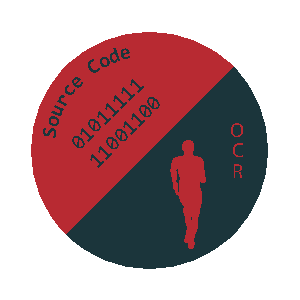
\includegraphics[width=0.35\textwidth]{images/logo.eps}
	% -----------------------
	\caption{Traditionelle Latexproduktion}\label{fig:latex}%
\end{figure}
\marginpar{Abb.}


\begin{lstlisting}[language=TeX,% C, TeX, Bash, Python
]-----Code einfügen---------------------------%
	% Optionen
	scale = Wert, Vergrösserungsfaktor
	width/height = Wert für die Einstellung der Breite/Höhe
	angle = Wert, Winkel (in Grad)
	b = bottom - Seitenende 
	t = top - Seitenanfang
	h = here
	p = page - komplette Seite  
	
	\begin{figure}[hb]
	\centering
	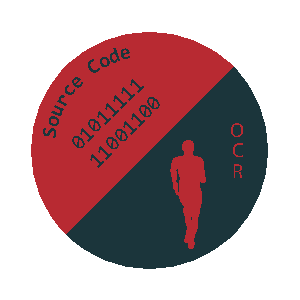
\includegraphics[width=0.35\textwidth]{images/logo.eps}
	% -----------------------
	\caption{Traditionelle Latexproduktion}\label{fig:latex}%
	\end{figure}
\end{lstlisting}


\clearpage
\section*{Methodik}

Unter Zuhilfenahme der Formeln~\ref{eq:ekin} und \ref{eq:impuls} werden wir diese Forschungslücke schließen.  \marginpar{Mathe}
$E_\mathrm{kin}$ ist die kinetische Energie, $m$ die Masse und $\vec{v}$ die Geschwindigkeit.

Wurzel
$\sqrt{2}$

Bruch
$\frac{Zähler}{Nenner}$

\begin{equation}
% -----------------------
\label{eq:ekin}% 
\sum E_\mathrm{kin} = \sum E'_\mathrm{kin}
\end{equation}

\begin{equation}
% -----------------------
\label{eq:impuls}% 
\vec{v_1} - \vec{v_1'} = \frac{m_2}{m_1} (\vec{v_2'} - \vec{v_2})
\end{equation}

\clearpage
\section*{Ausblick}

Daraus ergeben sich gemäß (\ref{tab:schritte}) folgende nächste Schritte, deren sequenzielle Ausführung von essenzieller Bedeutung ist.

\begin{table}[ht]
	\centering
	\begin{tabular}{ll}% lcr
		\toprule
		\textbf{Nr.} & \textbf{Vorgehen} \\
		\midrule
		1 & Aktuellen Forschungsstand recherchieren \\
		2 & Methoden entwickeln \\
		3 & Schlussfolgerung aufstellen \\
		\bottomrule
	\end{tabular}
	% -----------------------
	\caption{Nächste Schritte}\label{tab:schritte}
\end{table}
\marginpar{Tabelle} 

\begin{lstlisting}[language=TeX,% C, TeX, Bash, Python
]-----Code einfügen---------------------------%
	\begin{table}[ht]
	\centering
	\begin{tabular}{ll}% lcr
	\toprule
	\textbf{Nr.} & \textbf{Vorgehen} \\
	\midrule
	1 & Aktuellen Forschungsstand recherchieren \\
	2 & Methoden entwickeln \\
	3 & Schlussfolgerung aufstellen \\
	\bottomrule
	\end{tabular}
	% -----------------------
	\caption{Nächste Schritte}\label{tab:schritte}
	\end{table}
\end{lstlisting}
